
%%----------------------------------------%%
\begin{frame}[ctb!]
  \frametitle{Release Mechanisms}
  \begin{itemize} 
  \item Human Disruption
  \item Natural Disruption
  \item Barrier Dissolution
  \item Advection
  \item Diffusion
  \item Sorption
  \item Solubility Limitation
  \item ... 
  \end{itemize}
\end{frame}

%%----------------------------------------%%
\begin{frame}
\frametitle{Solubility Sensitivity In A Clay Model}
\begin{figure}[ht]
  \centering
  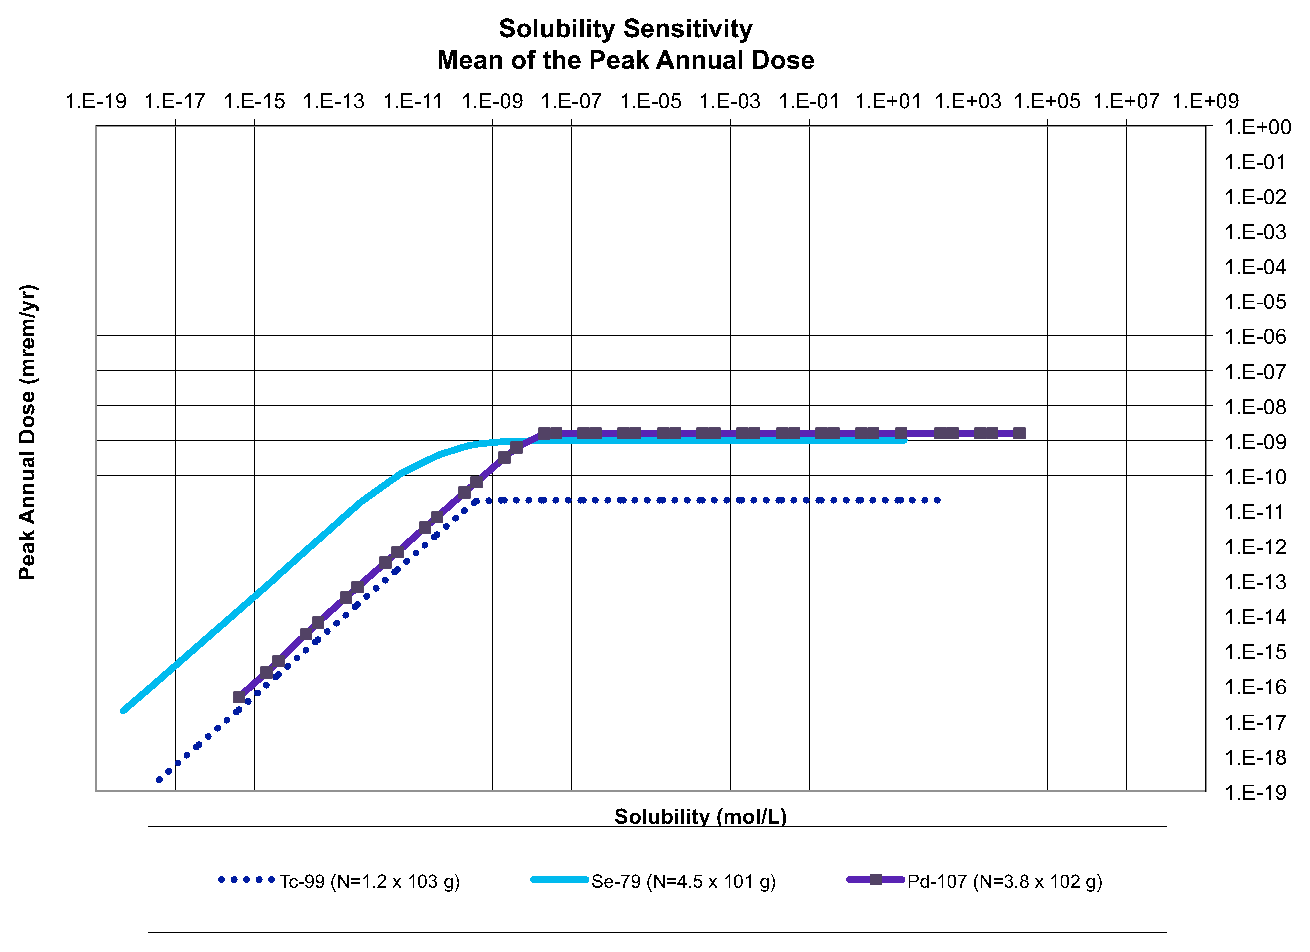
\includegraphics[width=0.7\linewidth]{Solubility_Summary.eps}
  \caption{Solubility limit sensitivity. The peak annual dose due to an 
  inventory, $N$, of each isotope.}
  \label{fig:SolSum}
\end{figure}
\end{frame}

%%----------------------------------------%%
\begin{frame}[ctb]
\frametitle{Retardation Sensitivity In A Clay Model}
\begin{figure}[ht]
  \centering
  \includegraphics[width=0.7\linewidth]{Partitioning_Summary.eps}
  \caption{$K_d$ sensitivity.  The peak annual dose due to an inventory, 
  $N$, of each isotope.}
  \label{fig:KdSum}
\end{figure}
\end{frame}

%%----------------------------------------%%
\begin{frame}[c]
  \frametitle{Example : Vertical Advective Velocity and Diffusion Coefficient}
\begin{figure}[htp!]
\centering
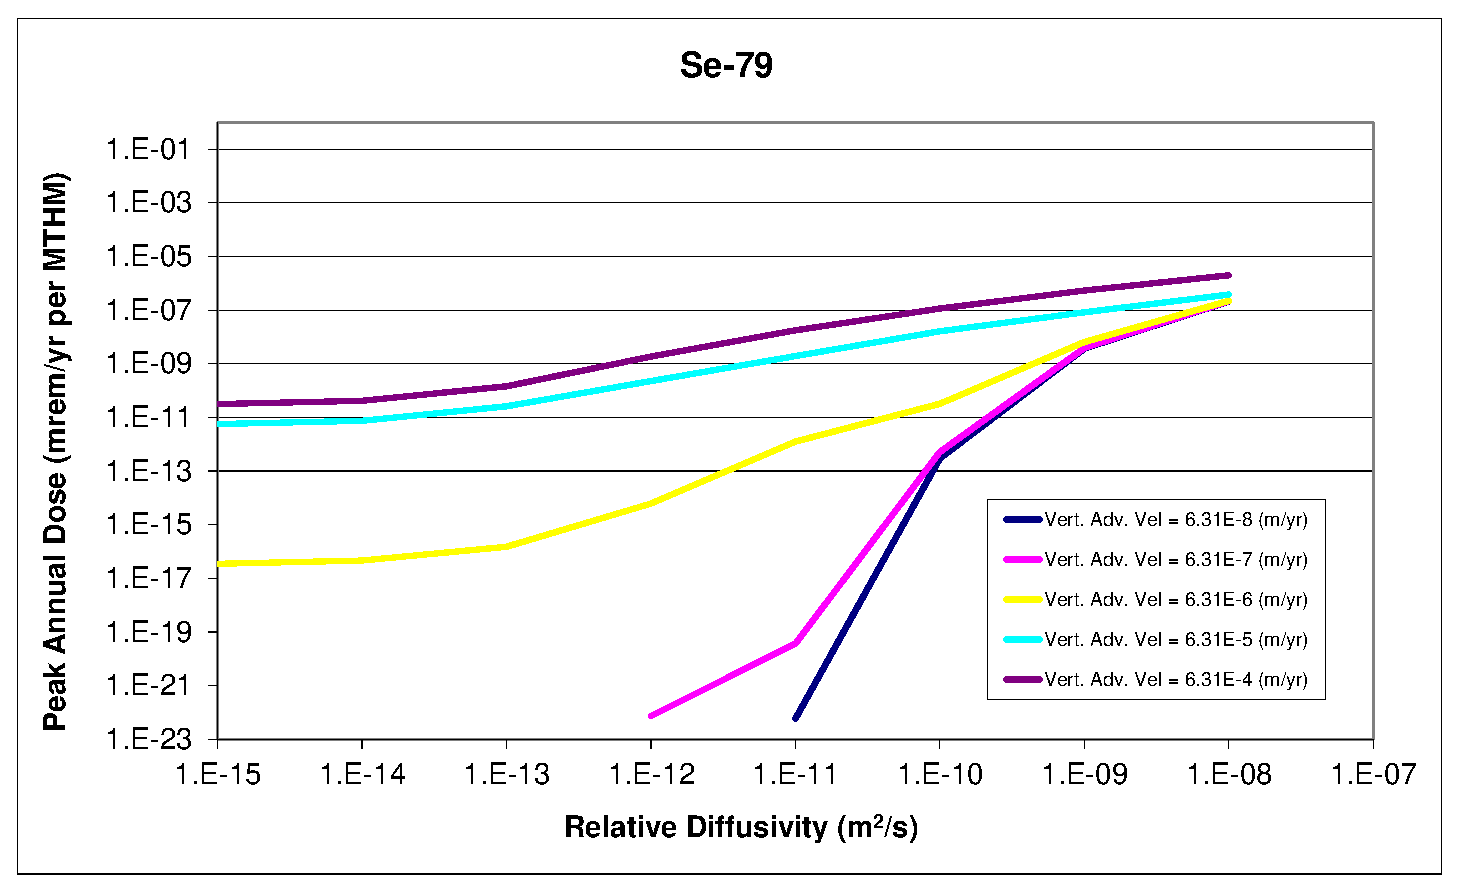
\includegraphics[width=0.8\textwidth]{Se-79.eps}
\caption{$^{79}Se$.  $Se$ is non sorbing, but solubility limited in clay.  For low vertical advective velocity, the system is diffusion dominated.}
\label{fig:VAdvVelSe79}
\end{figure}
\end{frame}

%%----------------------------------------%%
\begin{frame}[c]
  \frametitle{Example : Vertical Advective Velocity and Diffusion Coefficient}
\begin{figure}[ht!]
\centering
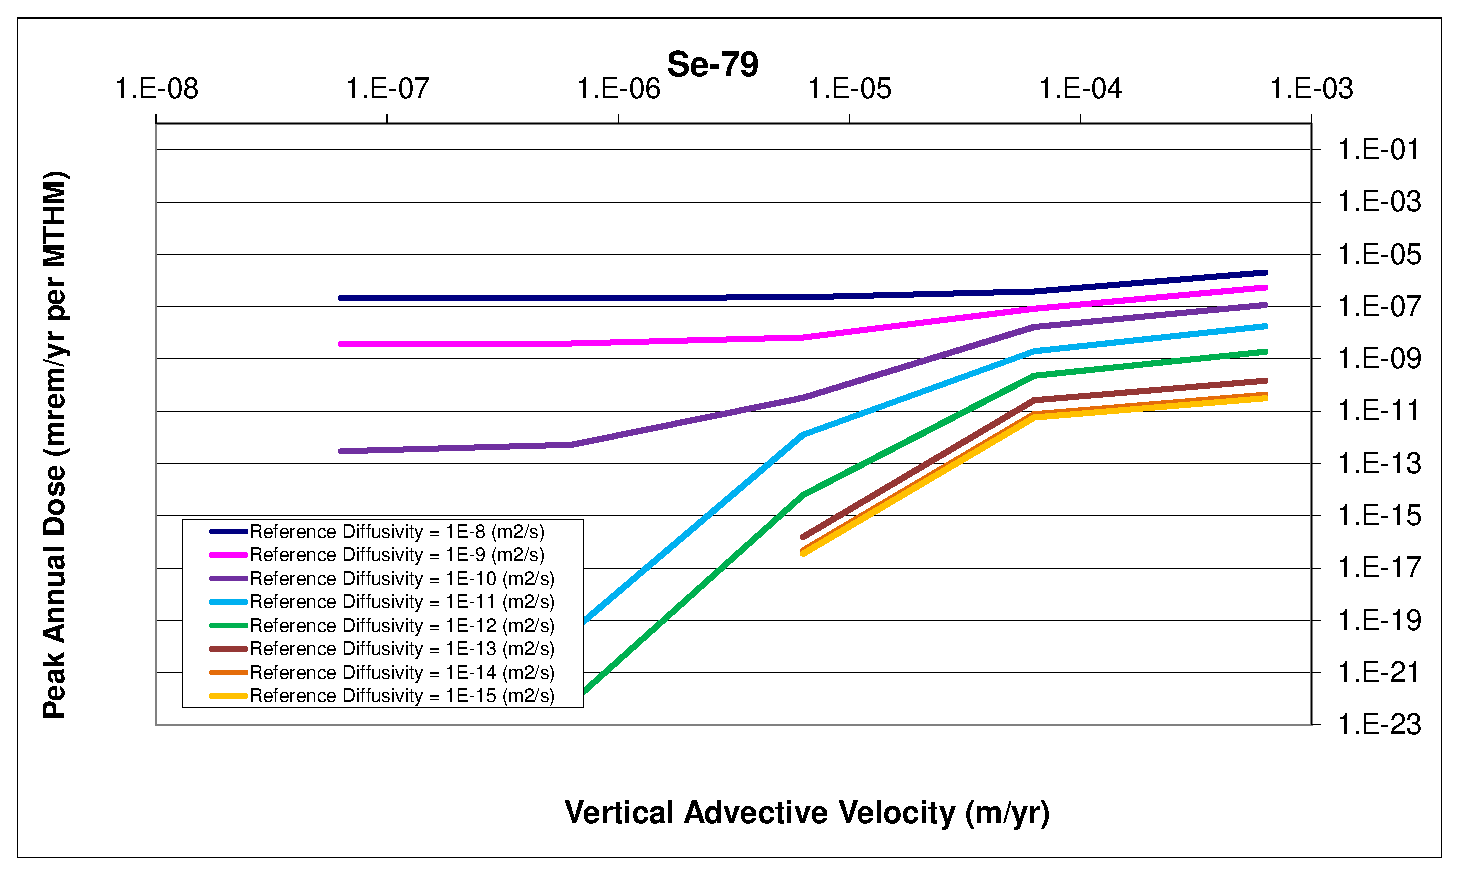
\includegraphics[width=0.8\textwidth]{Se-79-VAdvVel.eps}
\caption{$^{79}Se$.
$Se$ is non sorbing, but solubility limited in clay.
For high vertical advective 
velocity, the diffusivity remains important even in the advective regime as 
spreading facilitates transport in the presence of solubility limited 
transport.} 
\label{fig:VAdvVelSe79VAdvVel}
\end{figure}
\end{frame}

